% Using KOMA Script document style
% Font size setting and
% option to skip empty lines as new paragraphs
\documentclass[10pt,a4paper]{article}
% Packages without Options
\usepackage{
	algorithm,
	alltt,
	algpseudocode,
	amsfonts,
	amssymb,
	appendix,
	array,
	booktabs,
	dirtree,
	enumitem,
	float,
	footnote,
	gensymb,
	geometry,
	graphicx,
	interval,
	karnaugh-map,
	lipsum,
	listings,
	longtable,
	makecell,
	mathtools,
	minted,
  nicematrix,
	parskip,
	pdfpages,
	pgfkeys,
	pgfplots,
	subcaption,
	tabularx,
	tablefootnote,
	textcomp,
	tikz,
    titlecaps,
	venndiagram,
	wrapfig,
	wrapfig,
	xcolor
}



% Packages with Options

\usepackage[framemethod=tikz]{mdframed}
\usepackage[colorlinks,linkcolor=cyan, citecolor=cyan, urlcolor=cyan]{hyperref}
\usepackage[labelfont=bf,textfont=it,labelsep=period]{caption}
\usepackage[RPvoltages]{circuitikz}
\usepackage[english]{babel}
\usepackage[nameinlink,noabbrev]{cleveref}

\definecolor{mintedbackground}{rgb}{0.97,0.97,0.97}

\setminted[cpp]{
bgcolor=mintedbackground,
    linenos=true,
    breaklines=true,}

\setminted[js]{
bgcolor=mintedbackground,
    linenos=true,
    breaklines=true,}

\setminted[python]{
bgcolor=mintedbackground,
    linenos=true,
    breaklines=true,}
    

\linespread{1.5}

% Package: AlgorithmicX
% Sets all comments to be indentend and aligned

\renewcommand{\Comment}[2][.7\linewidth]{%
  \leavevmode\hfill\makebox[#1][l]{//~#2}}


% Package: Interval
% Sets the style of mathematical intervals
\intervalconfig{
soft open fences, separator symbol=,,
}

% Package: Geometry
% Sets the page margins
\geometry{
    a4paper,
    left=32mm,
    right=22mm,
    top=22mm,
    }
	
% Creates a proper caption name for algorithms
\newcommand{\algorithmautorefname}{Algorithm}
\newcommand{\listingautorefname}{Listing}
\algrenewcommand{\algorithmiccomment}[1]{\texttt{// #1} }
% Creates a numbered environment for Theorems
\newtheorem{theorem}{Theorem}

% Redefine the implication arrow to be a simple, thin arrow instead of the default, thick arrow
\renewcommand{\implies}{\rightarrow}

% Create a new command for the set complement to make my logical statements easier to read
\newcommand{\compl}{\overline}

% Creates commands for combinatorics nCr and nPr
\newcommand{\nCr}[2]{\,_{#1}C_{#2}} % nCr
\newcommand{\nPr}[2]{\,_{#1}P_{#2}} % nPr

% Package: tikz
% Loads libraries for drawing automata, 
\usetikzlibrary{automata,positioning,shadows,arrows, shapes.gates.logic.US, calc}

% Creates a command to create a button shape
\newcommand*\keystroke[1]{%
  \tikz[baseline= (key.base)]
    \node[%
      draw,
      fill=white,
      drop shadow={shadow xshift=0.25ex,shadow yshift=-0.25ex,fill=black,opacity=0.75},
      rectangle,
      rounded corners=2pt,
      inner sep=1pt,
      line width=0.5pt,
      font=\scriptsize\sffamily
    ] (key) {#1\strut};
}

% Package: pgfplot
% Sets the global options for PGF Plots
\pgfplotsset{compat=newest}

% Package: tikz
% Flowchart Shapes
\tikzstyle{startstop} = [rectangle, rounded corners, minimum width=3cm, minimum height=1cm,text centered, draw=black, fill=red!30]
\tikzstyle{io} = [trapezium, trapezium left angle=70, trapezium right angle=110, minimum width=3cm, minimum height=1cm, text centered, draw=black, fill=blue!30]
\tikzstyle{process} = [rectangle, minimum width=3cm, minimum height=1cm, text centered, draw=black, fill=orange!30]
\tikzstyle{decision} = [diamond, minimum width=3cm, minimum height=1cm, text centered, draw=black, fill=green!30]
\tikzstyle{arrow} = [thick,->,>=stealth]

% Disable Minted syntax error highlights (red boxes)
\AtBeginEnvironment{minted}{%
  \renewcommand{\fcolorbox}[4][]{#4}}

% Listings Style (non-minted)

\lstdefinestyle{arjuncode}{
    basicstyle=\ttfamily,
    breakatwhitespace=false,         
    breaklines=true,                 
    captionpos=b,                    
    keepspaces=true,                 
    numbers=left,                    
    numbersep=5pt,                  
    showspaces=false,                
    showstringspaces=false,
    showtabs=false,                  
    tabsize=2
}

\lstset{style=arjuncode}

\graphicspath{{images/}}

 %Adjust this based on where your Summary is stored
\title{CM2010: Software Design and Development \\ Mid-term assignment}
\author{Arjun Muralidharan}
\begin{document}

\maketitle
\newpage
\tableofcontents
\listoffigures
\listoftables
% \listofalgorithms

\newpage
\renewcommand{\subsubsectionautorefname}{section\negthinspace}

\section{Part 1: Module Coupling \& Cohesion} % (fold)
\label{sec:part_1_module_coupling_&_cohesion}
For this part of the assignment, we will inspect a Cryptocurrency Trading application created as part of the module ``CM2005: Object Oriented Programming'' in the degree.

\paragraph{Description \& Purpose} % (fold)
\label{par:description_&_purpose}
The trading application, called ``Merklerex'', attempts to create trades on a fictional cryptocurrency market with a starting capital of Bitcoin. The goal is to place orders, execute them, and generate a profit after stepping through several timeframes to execute trades.
The basic structure (for the explanations below) is that the application maintains a \texttt{Wallet} object, which holds the users current balance of cryptocurrency. 
\begin{itemize}
	\item A \texttt{CSVReader} class is used to extract data from a CSV file of orders.
	\item A \texttt{OrderBook} class ingests these orders and maintains them as an object.
	\item A \texttt{Merklebot} class contains all the automated logic to trade in an automated fashion, and adds orders to the \texttt{OrderBook} and resulting balance changes to the \texttt{Wallet}.
	\item Finally, a \texttt{MerkleMain} class contains all functionality to control the application via user interaction.
\end{itemize}

The next sections describe examples of cohesion and coupling among these four classes. The application contains other classes, but these are not in scope for this analysis.
% paragraph description_&_purpose (end)

\subsection{Cohesion} % (fold)
\label{ssub:cohesion}

% subsubsection cohesion (end)
\paragraph{Example 1: Functional Cohesion} % (fold)
\label{par:example_1_functional_cohesion}
We can find a good example of functional cohesion in the \texttt{Wallet} class. This module has the sole \textbf{function} of maintaining the user's currency wallet. It limits its functionality to managing currency, running checks against the wallet, and providing information about the wallet to other modules. This level of cohesion is well observable in the class's header file (\autoref{lis:funccohesion}), which shows that all the class functions are related to the same business function. I argue that this is a well-designed class as functional cohesion is desirable.
% paragraph example_1_functional_cohesion (end)Functional Cohesion:

\begin{listing}[h]
	\caption{Functional cohesion in Wallet class}
	\label{lis:funccohesion}
	\begin{minted}{cpp}
class Wallet
{
public:
	Wallet();

	/** Insert currency to the wallet. */
	void insertCurrency(const std::string& type, double amount);

	/** Remove currency from the wallet. */
	bool removeCurrency(const std::string& type, double amount);

	/** Check if the order can be fulfilled */
	bool canFulfillOrder(const OrderBookEntry& order);

	/** Check if the wallet contains this much currency or more. */
	bool containsCurrency(const std::string& type, const double amount = 0);

	/** Process the sale */
	void processSale(OrderBookEntry& sale);

	/** Generate a string representation of the wallet. */
	std::string toString();

	/** Get the balance of a specific currency */
	double checkBalance(const std::string& currency);

	/** Retrieve the currencies present in the wallet */
	std::map<std::string, double> getCurrencies();

	/** Get the value of the wallet in USDT */
	double getWalletValue(OrderBook& orderBook, std::string currentTime);

private:
	std::map<std::string, double> currencies;
	friend std::ostream& operator<<(std::ostream& os, Wallet& wallet);
};
	\end{minted}
\end{listing}


\paragraph{Example 2: Procedural Cohesion} % (fold)
\label{par:procedural_cohesion}
The \texttt{Merklebot} class displays a level of procedural cohesion. It executes various functions across different pieces of data while related to the overall process of running an automated trade. For example, this module creates market predictions based on market data, creates orders based on those predictions, executes those orders, and updates the \texttt{Wallet}. While this is \emph{logically cohesive}, the implementation here is not desirable as the module works on different data, and therefore the overall complexity is very high. It also generates logs, which is a different function overall. I've demonstrated this by picking two functions from this module (\autoref{lis:proccohesion}) that operate on very different data and perform different functions procedurally related. Interestingly, this property of procedural cohesion becomes apparent when looking at the module as a whole; however, when looking at only the public API of this module, it seems more logically and functionally cohesive and less procedural. The interface maintains a good level of cohesion, but I can improve the module by moving some aspects of public functions and most private functions to a different module.
% paragraph procedural_cohesion (end)
\begin{listing}[h]
	\caption{Procedrual cohesion in the Merklebot class}
	\label{lis:proccohesion}
	\begin{minted}{cpp}

double MerkleBot::simpleMovingAverage(const std::string& product, const int& timeframes, const OrderBookType& type)
{
	int observations{0};
	double sumObservations{0};
	std::string timeframe{currentTime};
	while (orderBook.orders.find(timeframe) != orderBook.orders.begin() && observations < timeframes)
	{
		std::vector<OrderBookEntry> orders{orderBook.getOrders(type, product, timeframe)};
		if (orders.size() > 0)
		{
			sumObservations += orders.back().price;
			timeframe = orderBook.getPreviousTime(timeframe);
			++observations;
		}
		else
		{
			timeframe = orderBook.getPreviousTime(timeframe);
		}
	}
	return sumObservations / timeframes;
}

//////////////

// R3A: Bot generates a log of the contents of its wallet
void MerkleBot::generateWalletLog()
{
	std::ofstream walletLog;
	walletLog.open("walletLog.txt");
	walletLog << wallet << std::endl;
	walletLog.close();
}
	\end{minted}
\end{listing}

\subsection{Coupling} % (fold)
\label{ssub:coupling}

% subsubsection coupling (end)
\paragraph{Example 1: Data coupling} % (fold)
\label{par:paragraph_name}
An example of data coupling, where one module provides the data input for the latter module, can be seen in how the \texttt{CSVReader} class provides input for the \texttt{OrderBook} class. Here, I've extracted the function that calls the \texttt{CSVReader} class, the function that creates the input data and how it is then processed in the original \texttt{OrderBook} class (\autoref{lis:datacoupling}).

% paragraph paragraph_name (end)

\begin{listing}[h]
	\caption{Procedrual cohesion in the Merklebot class}
	\label{lis:datacoupling}
	\begin{minted}{cpp}
// Calling the CSVReader class for data and processing it
OrderBook::OrderBook(const std::string& filename)
{
	std::cout << "Loading market data..." << std::endl;
	orders = CSVReader::readCSV(filename);
	std::cout << "Read " << orders.size() << " timestamps." << std::endl;
	products = getKnownProducts();
}

// Creating the data and sending back OrderBook entries
std::map<std::string, std::vector<OrderBookEntry>> CSVReader::readCSV(std::string csvFileName)
{
	std::map<std::string, std::vector<OrderBookEntry>> entries;
	std::ifstream csvFile{csvFileName};

	if (csvFile.is_open())
	{
		std::string line;
		while (std::getline(csvFile, line))
		{
			OrderBookEntry obe{stringsToOBE(tokenise(line, ','))};
			entries[obe.timestamp].push_back(obe);
		}
	}
	else
	{
		std::cout << "Problem opening file " << csvFileName << std::endl;
	}
	csvFile.close();
	return entries;
}

		\end{minted}
\end{listing}



\paragraph{Example 2: Content coupling} % (fold)
\label{par:example_2_content_coupling}
An example of content coupling is visible in the \texttt{MerkleMain} and \texttt{MerkleBot} classes, which operate on a common data area. They both access the \texttt{Wallet} as a data object and operate on it while doing different things with it. To demonstrate this coupling, I've extracted a function from each of these classes (\autoref{lis:contentcoupling}) that operate on the same data. In this case, this kind of coupling is fairly safe, as the data is not in a global space and passed from one module to the other in a controlled, one-way manner.
% paragraph example_2_content_coupling (end)
\begin{listing}[h]
	\caption{Content coupling in the MerkleMain and MerkleBot classes}
	\label{lis:contentcoupling}
	\begin{minted}{cpp}
// MerkleBot operating on the wallet data
void MerkleBot::executeTrades()
{
	for (const std::string& product : orderBook.products)
	{
		std::vector<OrderBookEntry> sales = orderBook.matchAsksToBids(product, currentTime);

		for (OrderBookEntry& sale : sales)
		{
			if (sale.username == "simuser" && wallet.canFulfillOrder(sale))
			{
				wallet.processSale(sale);
				generateBidsAsksSalesLog(sale);
			}
		}
	}
}


// MerkleMain operating on the wallet data
void MerkleMain::init()
{
	currentTime = orderBook.orders.begin()->first;
	short int input;
	wallet.insertCurrency("BTC", 10);
	wallet.insertCurrency("ETH", 100);
	wallet.insertCurrency("DOGE", 1000);

	// ...
}
	\end{minted}
\end{listing}
% section part_1_module_coupling_&_cohesion (end)

\section{Part 2: Unit Testing Activity} % (fold)
\label{sec:part_2_unit_testing_activity}

For this part of the assignment, I chose the \texttt{norestforthewiccad} RESTful API for which to write tests. I used the MochaJS and ChaiJS frameworks for these tests. 

\subsection{Scope}
I decided to design a test for CRUD-style operations, testing for the applications capability to successfully \textbf{read}, \textbf{update} and \textbf{create} records via the API. These three operations are the foundation of the three test sets created.

The tests attempt to facilitate the development of these basic operations but do not seek full coverage of edge cases and failures that may occur, especially data integrity. The tests assume the limited number of spells available in the source data. Further development would be needed to test against a large set of data, and I could employ more sophisticated testing strategies to handle test data.

\subsection{Test Set 1: Read --- \texttt{GET /spells}}

\paragraph{Strategy} I decided first to ensure that the \texttt{spells} endpoint returns successfully when the application places a GET request against it. I then decided to extend functionality by checking that the response contained spells with the correct number of attributes that a spell should have. Finally, I decided to build functionality to retrieve a specific spell and make sure that the returned spell is indeed the one I had requested. This strategy allowed gradually building out the endpoint's data model and retrieving more specific data with each test. It also ensured that we first built functional middleware before populating it with business logic.

\subparagraph{Test Set 1, Test 1} This test checks for the endpoints response code and expects a successful response, as shown in \autoref{lis:test1_1}.

\begin{listing}[h]
\caption{Test Set 1, Test 1}
\label{lis:test1_1}

\begin{minted}{js}
// The /spells route should be reached successfully
describe("Get everything at /spells", () => {
	it("should return successfully", (done) => {
		chai.request(app)
			.get("/spells")
			.end((err, res) => {
				assert.equal(res.status, 200);
				done();
			});
	});
});
\end{minted}
\end{listing}

The before and after test output is visible in \autoref{fig:test1_1}.

\begin{figure}[h]
\caption{Test output for test set 1, test 1}
\label{fig:test1_1}
	\centering
	\begin{subfigure}[b]{0.5\textwidth}
		\centering
		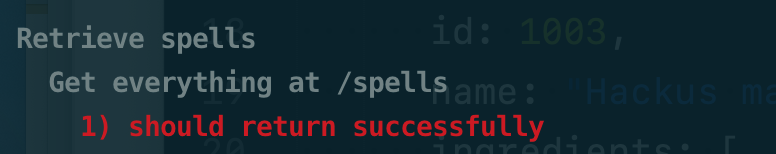
\includegraphics[width=\textwidth]{images/11_fail}
		\caption{Fail}
		\label{fig:test11_fail}
	\end{subfigure}
	\hfill
	\begin{subfigure}[b]{0.5\textwidth}
		\centering
		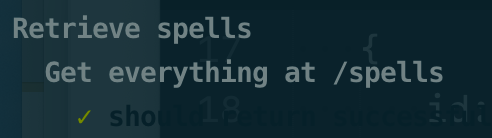
\includegraphics[width=\textwidth]{images/11_pass}
		\caption{Pass}
		\label{fig:test11_pass}
	\end{subfigure}
\end{figure}

\subparagraph{Test Set 1, Test 2} This test checks if the response consists of an array of objects, each with precisely four attributes. To make this test pass, I had to return the full contents of the \texttt{spells} array and then check for it by iterating over each spell and counting the number of keys. We also check that the body of the response is, in fact, an array, as shown in \autoref{lis:test1_2}

\begin{listing}[h]
\caption{Test Set 1, Test 2}
\label{lis:test1_2}
\begin{minted}{js}
describe("Ensure spells are spells with correct length", () => {
	it("should return spells with proper length", (done) => {
		chai.request(app)
			.get("/spells")
			.end((err, res) => {
				assert.typeOf(res.body, 'array');
				assert.isAtLeast(res.body.length, 1);
				for (var i = 0; i < res.body.length; i++) {
					assert.lengthOf(Object.keys(res.body[i]), 4);
				}
				done();
			});
	});
});
\end{minted}
\end{listing}

The before and after test output is visible in \autoref{fig:test1_2}.

\begin{figure}[h]
\caption{Test output for test set 1, test 2}
\label{fig:test1_2}
	\centering
	\begin{subfigure}[b]{0.5\textwidth}
		\centering
		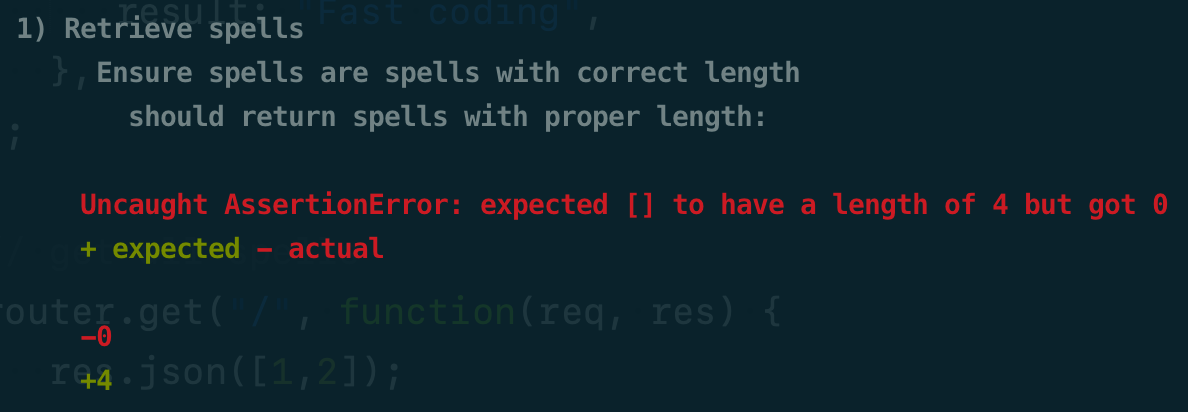
\includegraphics[width=\textwidth]{images/12_fail}
		\caption{Fail}
		\label{fig:test12_fail}
	\end{subfigure}
	\hfill
	\begin{subfigure}[b]{0.5\textwidth}
		\centering
		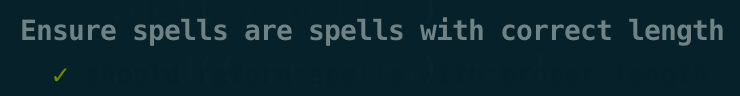
\includegraphics[width=\textwidth]{images/12_pass}
		\caption{Pass}
		\label{fig:test12_pass}
	\end{subfigure}
\end{figure}


\subparagraph{Test Set 1, Test 3} The final test in this set requests a specific spell by passing an additional parameter to the route at \texttt{/spells/:id} and checks if the returned spell has the same ID as was requested, as shown in \autoref{lis:test1_3}.

\begin{listing}[h]
\caption{Test Set 1, Test 3}
\label{lis:test1_3}
\begin{minted}{js}
describe("Get a specific spell", () => {
	// Configure a specific spell to test for
	let testId = "1001";
	it("should return the correct spell that was requested", (done) => {
		chai.request(app)
			.get("/spells/" + testId)
			.end((err, res) => {
				assert.equal(res.body.id, testId);
				done();
			});
	});
});

\end{minted}
\end{listing}
The before and after output of this test is shown in \autoref{fig:test1_3}.
\begin{figure}[h]
\caption{Test output for test set 1, test 3}
\label{fig:test1_3}
	\centering
	\begin{subfigure}[b]{0.5\textwidth}
		\centering
		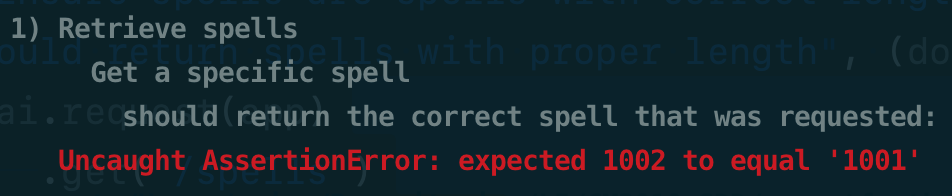
\includegraphics[width=\textwidth]{images/13_fail}
		\caption{Fail}
		\label{fig:test13_fail}
	\end{subfigure}
	\hfill
	\begin{subfigure}[b]{0.5\textwidth}
		\centering
		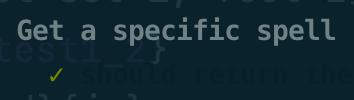
\includegraphics[width=\textwidth]{images/13_pass}
		\caption{Pass}
		\label{fig:test13_pass}
	\end{subfigure}
\end{figure}

\subsection{Test Set 2: Update --- \texttt{PUT /spells/:id}}

\paragraph{Strategy} For this set of tests, I decided to progressively test updating a spell, first by trying to place a successful \texttt{PUT} request against a specific spell ID and then trying to edit a single attribute, followed by updating the entirety of a spell. Again, this allowed me to gradually expand the data model of this function as I tested.

\subparagraph{Test Set 2, Test 1} This test checks for the endpoints response code and expects a successful response, as shown in \autoref{lis:test2_1}.

\begin{listing}[h]
\caption{Test Set 2, Test 1}
\label{lis:test2_1}

\begin{minted}{js}
// The /spells route should be reached successfully
describe("Send an update request successfully", () => {
	let testId = "1003";
	it("should update a spell", (done) => {
		chai.request("http://localhost:3000")
			.put("/spells/" + testId)
			.end((err, res) => {
				assert.equal(res.status, 200);
				done();
			});
	});
});
\end{minted}
\end{listing}

The before and after test output is visible in \autoref{fig:test2_1}.

\begin{figure}[h]
\caption{Test output for test set 2, test 1}
\label{fig:test2_1}
	\centering
	\begin{subfigure}[b]{0.5\textwidth}
		\centering
		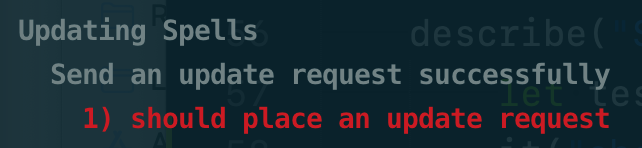
\includegraphics[width=\textwidth]{images/21_fail}
		\caption{Fail}
		\label{fig:test21_fail}
	\end{subfigure}
	\hfill
	\begin{subfigure}[b]{0.5\textwidth}
		\centering
		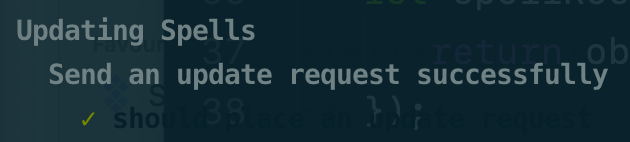
\includegraphics[width=\textwidth]{images/21_pass}
		\caption{Pass}
		\label{fig:test21_pass}
	\end{subfigure}
\end{figure}

\subparagraph{Test Set 2, Test 2} This test tries to update the name of an existing spell by sending that attribute via a \texttt{PUT} request and checking if the updated spell, retrieved by ID, does have an updated name, as shown in \autoref{lis:test2_2}.

\begin{listing}[h]
\caption{Test Set 2, Test 2}
\label{lis:test2_2}
\begin{minted}{js}
describe("Update the name of a spell", () => {
	let testId = 1003;
	let newName = "Hackus maximus";
	it("should update a single attribute of a spell", (done) => {
		chai.request("http://localhost:3000")
			.put("/spells/" + testId)
			.send({ name: newName })
			.end((err, res) => {
				assert.equal(res.body.name, newName);
				done();
			});
	});
});
\end{minted}
\end{listing}

The before and after test output is visible in \autoref{fig:test2_2}.

\begin{figure}[h]
\caption{Test output for test set 2, test 2}
\label{fig:test2_2}
	\centering
	\begin{subfigure}[b]{0.5\textwidth}
		\centering
		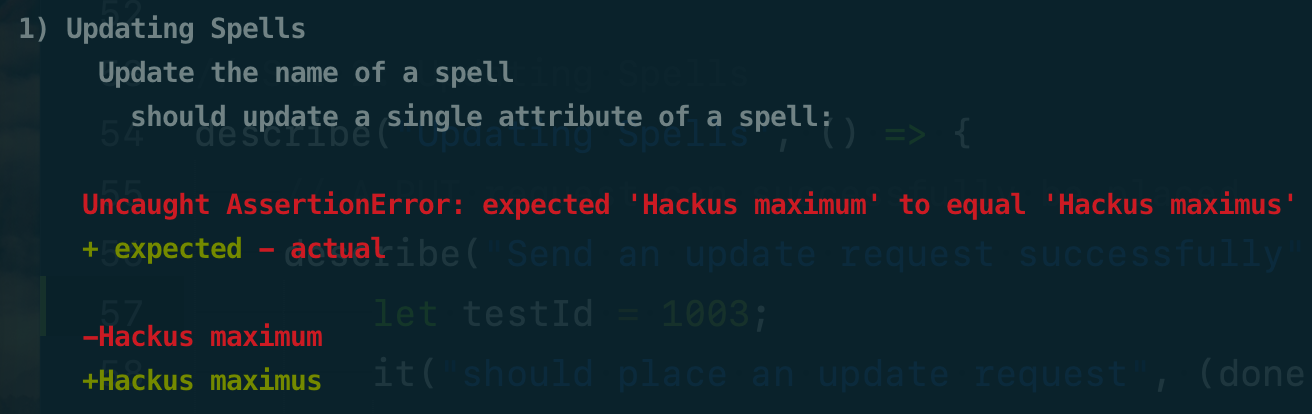
\includegraphics[width=\textwidth]{images/22_fail}
		\caption{Fail}
		\label{fig:test22_fail}
	\end{subfigure}
	\hfill
	\begin{subfigure}[b]{0.5\textwidth}
		\centering
		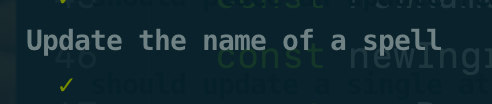
\includegraphics[width=\textwidth]{images/22_pass}
		\caption{Pass}
		\label{fig:test22_pass}
	\end{subfigure}
\end{figure}


\subparagraph{Test Set 2, Test 3} The test expands on the previous test and attempts to update all fields of a specific spell, as shown in \autoref{lis:test2_3}.

\begin{listing}[h]
\caption{Test Set 2, Test 3}
\label{lis:test2_3}
\begin{minted}{js}
describe("Update multiple fields of a spell", () => {
	let testId = 1003;
	let updatedName = "Hackus maximus";
	let updatedIngredients = [
		{ name: "Stroustrup hair" },
		{ name: "Uncle Bob sweat" },
	];
	let updatedResult = "Clean coding";
	let updatedSpell = {
		id: testId,
		name: updatedName,
		ingredients: updatedIngredients,
		result: updatedResult,
	};
	it("should update multiple fields of a spell", (done) => {
		chai.request("http://localhost:3000")
			.put("/spells/" + testId)
			.send(updatedSpell)
			.end((err, res) => {
				assert.equal(
					JSON.stringify(res.body),
					JSON.stringify(updatedSpell)
				);
				done();
			});
	});
});

\end{minted}
\end{listing}
The before and after output of this test is shown in \autoref{fig:test2_3}.
\begin{figure}[h]
\caption{Test output for test set 2, test 3}
\label{fig:test2_3}
	\centering
	\begin{subfigure}[b]{0.5\textwidth}
		\centering
		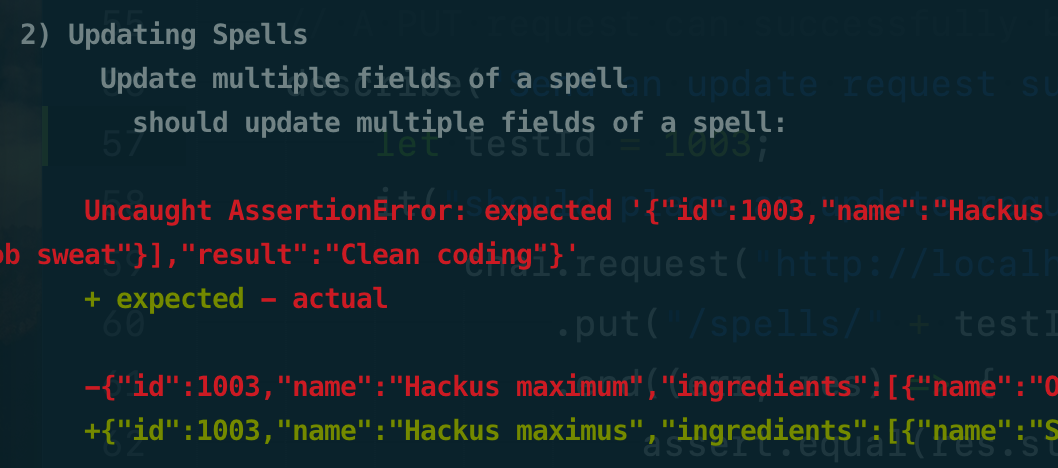
\includegraphics[width=\textwidth]{images/23_fail}
		\caption{Fail}
		\label{fig:test23_fail}
	\end{subfigure}
	\hfill
	\begin{subfigure}[b]{0.5\textwidth}
		\centering
		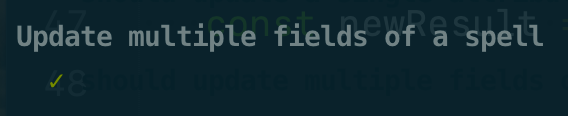
\includegraphics[width=\textwidth]{images/23_pass}
		\caption{Pass}
		\label{fig:test23_pass}
	\end{subfigure}
\end{figure}




\subsection{Test Set 3: Write --- \texttt{POST /spells}}
\paragraph{Strategy} For the third set of tests, I attempt to create a new spell and store it in the application's memory. I again attempt to gradually build this new dummy spell with just an ID and check if the application created the spell with that ID. I then expand on this to add more fields in a new spell and check that I cannot create a spell if another spell with the same ID already exists (duplicate prevention).

\subparagraph{Test Set 3, Test 1} This test places a \texttt{POST} request with a spell that only has an ID field. It checks if it can create the spell and if it gets returned correctly, as shown in \autoref{lis:test3_1}.

\begin{listing}[h]
\caption{Test Set 3, Test 1}
\label{lis:test3_1}

\begin{minted}{js}
// The /spells route should be reached successfully
describe("Add a basic spell with an ID", () => {
	let newId = 1004;
	it("should add a spell with an ID", (done) => {
		chai.request("http://localhost:3000")
			.post("/spells/")
			.send({ id: newId })
			.end((err, res) => {
				assert.equal(res.status, 200);
				assert.equal(res.body.id, newId);
				done();
			});
	});
});
\end{minted}
\end{listing}

The before and after test output is visible in \autoref{fig:test3_1}.

\begin{figure}[h]
\caption{Test output for test set 3, test 1}
\label{fig:test3_1}
	\centering
	\begin{subfigure}[b]{0.5\textwidth}
		\centering
		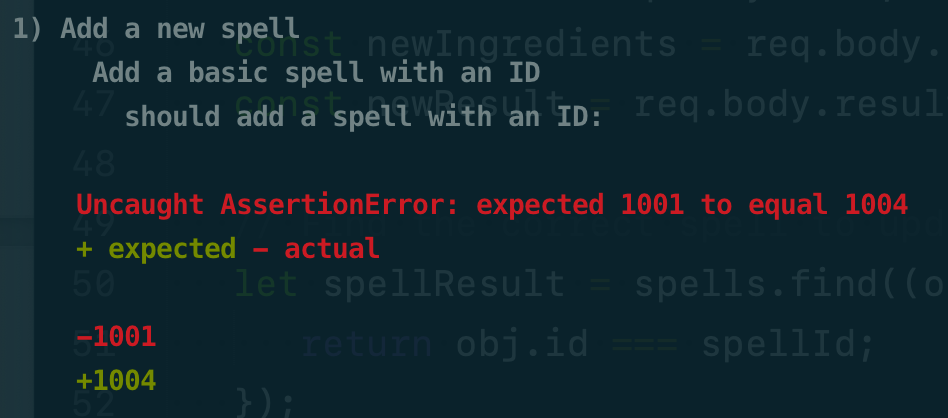
\includegraphics[width=\textwidth]{images/31_fail}
		\caption{Fail}
		\label{fig:test31_fail}
	\end{subfigure}
	\hfill
	\begin{subfigure}[b]{0.5\textwidth}
		\centering
		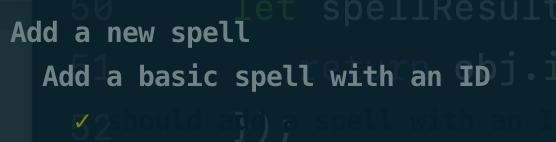
\includegraphics[width=\textwidth]{images/31_pass}
		\caption{Pass}
		\label{fig:test31_pass}
	\end{subfigure}
\end{figure}

\subparagraph{Test Set 3, Test 2} This test goes further by adding more fields to the spell created and ensures that the returned spell is identical to the one I wanted to create, as shown in \autoref{lis:test3_2}.

\begin{listing}[h]
\caption{Test Set 3, Test 2}
\label{lis:test3_2}
\begin{minted}{js}
describe("Add a spell with the right number of fields", () => {
	let newSpell = {
		id: 1005,
		name: "Wingardium Leviosa",
		ingredients: [{ name: "Bird blood" }, { name: "Feather essence" }],
		result: "Dream of Flight",
	};
	it("should add all fields to the spell correctly", (done) => {
		chai.request("http://localhost:3000")
			.post("/spells/")
			.send(newSpell)
			.end((err, res) => {
				assert.equal(
					JSON.stringify(res.body),
					JSON.stringify(newSpell)
				);
				assert.equal(Object.keys(res.body).length, 4);
				done();
			});
	});
});
\end{minted}
\end{listing}

The before and after test output is visible in \autoref{fig:test3_2}.

\begin{figure}[h]
\caption{Test output for test set 3, test 2}
\label{fig:test3_2}
	\centering
	\begin{subfigure}[b]{0.5\textwidth}
		\centering
		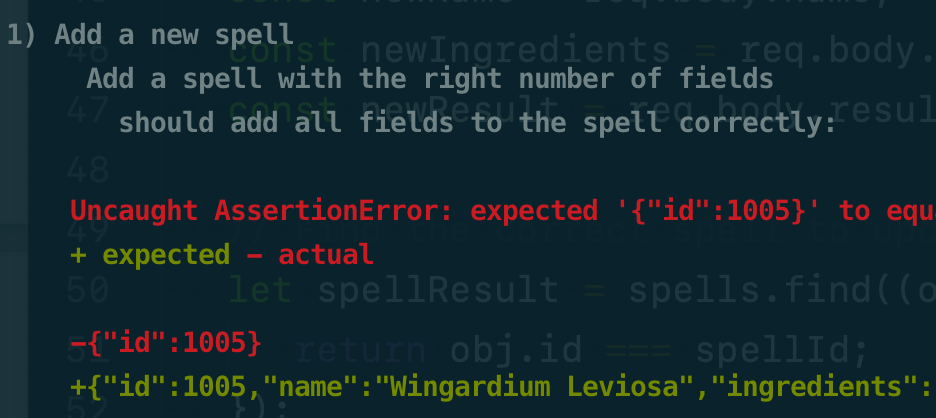
\includegraphics[width=\textwidth]{images/32_fail}
		\caption{Fail}
		\label{fig:test32_fail}
	\end{subfigure}
	\hfill
	\begin{subfigure}[b]{0.5\textwidth}
		\centering
		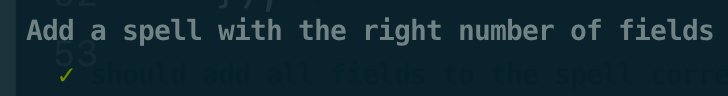
\includegraphics[width=\textwidth]{images/32_pass}
		\caption{Pass}
		\label{fig:test32_pass}
	\end{subfigure}
\end{figure}


\subparagraph{Test Set 3, Test 3} The final test tries to add a spell that already exists in the application, with the goal that this should not create a duplicate also not produce any error, as shown in \autoref{lis:test3_3}.

\begin{listing}[h]
\caption{Test Set 3, Test 3}
\label{lis:test3_3}
\begin{minted}{js}
describe("Attempt to add a duplicate spell", () => {
	// Create a duplicate spell object
	let newSpell = {
		id: 1001,
		name: "Rabbit foot positivity",
		ingredients: [
			{ name: "Foot of rabbit" },
			{ name: "Juice of beetle" },
		],
		result: "Good luck",
	};
	it("should return spells with unique IDs", (done) => {
		// Attempt to create the spell
		chai.request("http://localhost:3000")
			.post("/spells/")
			.send(newSpell)
			.end(() => {
				// Get all spells
				chai.request("http://localhost:3000")
					.get("/spells/")
					.end((err, res) => {
						// Cast the list of spells as a set
						// to get unique spells
						let spellSet = new Set(res.body);
						assert.equal(
							spellSet.size,
							res.body.length
							);
						done();
					});
			});
	});
});

\end{minted}
\end{listing}
The before and after output of this test is shown in \autoref{fig:test3_3}.
\begin{figure}[h]
\caption{Test output for test set 3, test 3}
\label{fig:test3_3}
	\centering
	\begin{subfigure}[b]{0.5\textwidth}
		\centering
		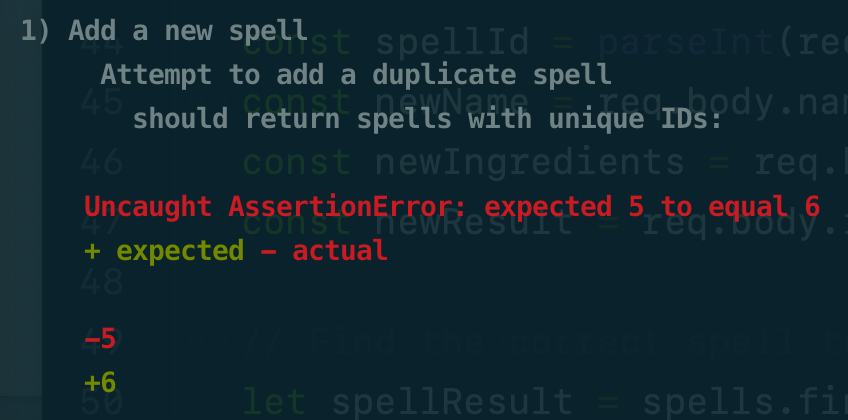
\includegraphics[width=\textwidth]{images/33_fail}
		\caption{Fail}
		\label{fig:test33_fail}
	\end{subfigure}
	\hfill
	\begin{subfigure}[b]{0.5\textwidth}
		\centering
		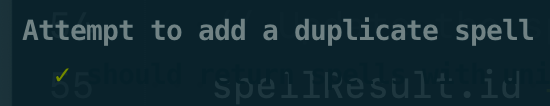
\includegraphics[width=\textwidth]{images/33_pass}
		\caption{Pass}
		\label{fig:test33_pass}
	\end{subfigure}
\end{figure}




% section part_2_unit_testing_activity (end)


\section{Part 3: Secure Programming} % (fold)
\label{sec:part_3_secure_programming}

For this part of the assignment, we will again use the Merklerex application used in part 1 and describe strategies for improving the application's security.

\subsection{Validating input files} % (fold)
\label{sub:validating_input_files}

As described in \cite{wheeler_2015}, all inputs to a program should be validated, especially when loaded from an external source or when the input is dynamic. In the Merklerex application, an external CSV file is loaded. The problem is that the CSV file contents are not checked, and assumptions about its format are made in the code. The code could easily inject undesirable code or data into the application at runtime. It can also cause the program to crash just by providing an unreasonably large file.
To solve this problem, we can employ the following strategy.
\begin{itemize}
	\item Use assertions to validate the size and format of the incoming CSV file.
	\item In the \texttt{CSVReader} class, check the file name and descriptors to ensure that the file is a CSV file. Some of this may already be provided by the CSV functions used in the program.
	\item When reading the CSV file lines, use \textbf{regular expressions} to validate that the file contents are of the correct format.
	\item Set limits to the file's possible size and check for this file as the file is loaded and as lines of the CSV are read. For example, ensure that the file does not get loaded if it exceeds 100MB, and stop loading lines after the first 10.000 lines have been read in.
	\item If such a scenario is encountered, use \textbf{exception handling} to treat those cases and degrade gracefully. For example, continue executing with fewer data and inform the user of this constraint.
\end{itemize}

All of these changes can happen in the \texttt{readCSV} function of this class.

% subsection validating_input_files (end)

\subsection{Minimize access to data} % (fold)
\label{sub:minimize_access_to_data}
According to \cite{wheeler_2015}, applications should minimize accessible data. The \texttt{OrderBook} class of the application exposes a map of \texttt{orders} and a set of \texttt{products} that are exposed as public data members. The problem with this is that any module can directly access these data members and manipulate them. It also directly exposes the type and implementation details of these two data members. No validation is done when changing any data within these members. A strategy for remediation might include:

\begin{itemize}
	\item Creating getter and setter functions for these data members and moving them to the private members of the \texttt{OrderBook} class.
	\item Incorporating validation for the setter functions to ensure that any data changes are legal. For example, if a product needs to be added to the list of products, ensure that it has the correct format, such as no numbers in the currency name, and at least one forward character to separate a currency pair such as ``BTC/USD''.
\end{itemize}

These changes require analyzing which functions in the applications access these data members and determine what kind of validation is needed. The benefit of doing this includes exposing which parts of the application change data vs. just reading from it, allowing for better control of module coupling.
% subsection minimize_access_to_data (end)

\subsection{Prevent buffer overflows} % (fold)
\label{sub:prevent_buffer_overflows}
The application makes certain assumptions about the size and sanity of variables. For example, numerous variables are declared of type \texttt{int} where it is assumed that the application will not encounter more than a certain number of orders in the source data. These variables could run into an overflow situation and cause serious errors or allow exploitation. A strategy to mitigate these would be:

\begin{itemize}
	\item Create assertions to check that variables stay within certain ranges.
	\item Use more flexible data types such as \texttt{auto} for unknown size variables before runtime.
	\item Implement exception handling so that the program can continue with a reduced set of data in the case of an overflow situation.
\end{itemize}
% subsection prevent_buffer_overflows (end)

% section part_3_secure_programming (end)


\bibliography{bib} 
\bibliographystyle{IEEEtran}

\end{document}

